% ============================================================
%  Apresentação: Modelagem e Controle de VANT (Quadricóptero)
%  Baseada em: "UAV Modelling and Control" (A. J. Peixoto)
%  e no documento main.tex do projeto
%  Compilar: pdflatex apresentacao.tex (2x)
% ============================================================
\documentclass[aspectratio=169, 11pt]{beamer}

% ---------- Tema e cores (modifique a gosto) ----------
\usetheme{Madrid}
\usecolortheme{default}
\setbeamertemplate{navigation symbols}{}      % remove ícones de navegação
\setbeamertemplate{caption}[numbered]

% ---------- Pacotes ----------
\usepackage[T1]{fontenc}
\usepackage[utf8]{inputenc}
\usepackage[brazilian]{babel}
\usepackage{lmodern}
\usepackage{amsmath, amssymb}
\usepackage{booktabs}
\usepackage{graphicx}
\usepackage{listings}                        % troque por minted se preferir
\usepackage{minted}
\lstset{
  basicstyle=\ttfamily\footnotesize,
  frame=single,
  breaklines=true,
  language=Python
}

% ---------- Metadados ----------
\title[Modelagem e Controle de VANT]{Modelagem Dinâmica e Controle de um VANT}
\subtitle{Rastreamento de trajetória e rejeição de perturbações}
\author[Kauan Moraes]{
  Kauan Moraes \\ 
  Prof. Dr. Alessandro Jacoud
}
\institute[]{Universidade Federal do Rio de Janeiro} % TODO: instituição / curso

\date[Oct 7]{October 7, 2026} % TODO: ajuste a data da apresentação

\begin{document}

% ============================================================
% ABERTURA
% ============================================================
\begin{frame}
  \titlepage
\end{frame}

\begin{frame}{Roteiro}
  \tableofcontents
\end{frame}

% ============================================================
% 1. INTRODUÇÃO
% ============================================================
\section{Introdução}

\begin{frame}{Motivação e Objetivos}
  \begin{block}{Objetivo geral}
    Modelar as forças e torques atuantes no VANT e desenvolver um sistema de
    controle capaz de \textbf{rastrear trajetórias de referência} e
    \textbf{rejeitar perturbações}, com arquitetura baseada no modelo dinâmico
    do veículo e validação em simulação.
  \end{block}
  \begin{itemize}
    \item % TODO: motivação (por que drones? aplicação alvo?)
    \item % TODO: contexto do trabalho (disciplina, projeto, parceria)
  \end{itemize}
  % TODO: figura do drone / foto do VANT
\end{frame}

% ============================================================
% 2. MODELAGEM
% ============================================================
\section{Modelagem}

\begin{frame}{Referenciais e Notação}
  \begin{itemize}
    \item Referencial inercial $\mathcal{E}_0$ e referencial do corpo $\mathcal{E}_b$.
    \item Matriz de rotação $R$: do corpo para o inercial.
    \item $\Omega = [\Omega_x, \Omega_y, \Omega_z]^T$: velocidade angular no corpo.
    \item % TODO: completar notação conforme o livro (massa M, inércias Ja, Jb, etc.)
  \end{itemize}
  % TODO: figura com os referenciais (cap. 1 do livro)
\end{frame}

\begin{frame}{Dinâmica de Translação}
  Formulação de Newton--Euler no referencial inercial, com compensação de
  gravidade, empuxo e arrasto:
  \begin{equation}
    \mathcal{M}\dot{v} = -\mathcal{M}g\,e_3 + R\,f\,e_3 + F_{\text{drag}}
  \end{equation}
  \begin{itemize}
    \item $\mathcal{M}$: massa total do VANT; \quad $f$: empuxo total comandado.
    \item $F_{\text{drag}}$: arrasto aerodinâmico (estrutura + rotores).
  \end{itemize}
  % TODO: mencionar modelos de arrasto do livro (H-force, arrasto quadrático)
\end{frame}

\begin{frame}{Dinâmica de Rotação}
  \begin{equation}
    J_b\,\dot{\Omega} = -(\Omega \times J_a\,\Omega) + M + \tau_{\text{drag}} + \tau_{\text{dist}}
  \end{equation}
  \begin{itemize}
    \item $J_a$, $J_b$: tensores de inércia dependentes de parâmetros físicos do drone.
    \item $M = [M_x, M_y, M_z]^T$: momentos gerados pelos controladores.
  \end{itemize}
  Cinemática de orientação ($J_R^{-1}$):
  \begin{equation}
    \begin{bmatrix} \dot{\phi} \\ \dot{\theta} \\ \dot{\psi} \end{bmatrix} =
    \begin{bmatrix}
      1 & \sin\phi\tan\theta & \cos\phi\tan\theta \\
      0 & \cos\phi           & -\sin\phi \\
      0 & \frac{\sin\phi}{\cos\theta} & \frac{\cos\phi}{\cos\theta}
    \end{bmatrix}
    \begin{bmatrix} \Omega_x \\ \Omega_y \\ \Omega_z \end{bmatrix}
  \end{equation}
  Evolução da matriz de rotação: $\dot{R} = R\hat{\Omega}$.
\end{frame}

\begin{frame}{Hipóteses e Aproximações}
  \begin{itemize}
    \item Baixas velocidades de translação $\Rightarrow$ simplificação dos arrastos.
    \item Ângulos pequenos: roll $\phi$ e pitch $\theta$ restritos (ex.: $< 15^\circ$).
    \item $\Omega \approx [\dot\phi, \dot\theta, \dot\psi]^T$ sob ângulos pequenos.
    \item Inércia constante. % TODO: referenciar pág. 9 do livro
  \end{itemize}
\end{frame}

% ============================================================
% 3. CONTROLE
% ============================================================
\section{Controle}
\label{sec:controle}
\begin{frame}{Arquitetura de Controle}
    \begin{figure}
    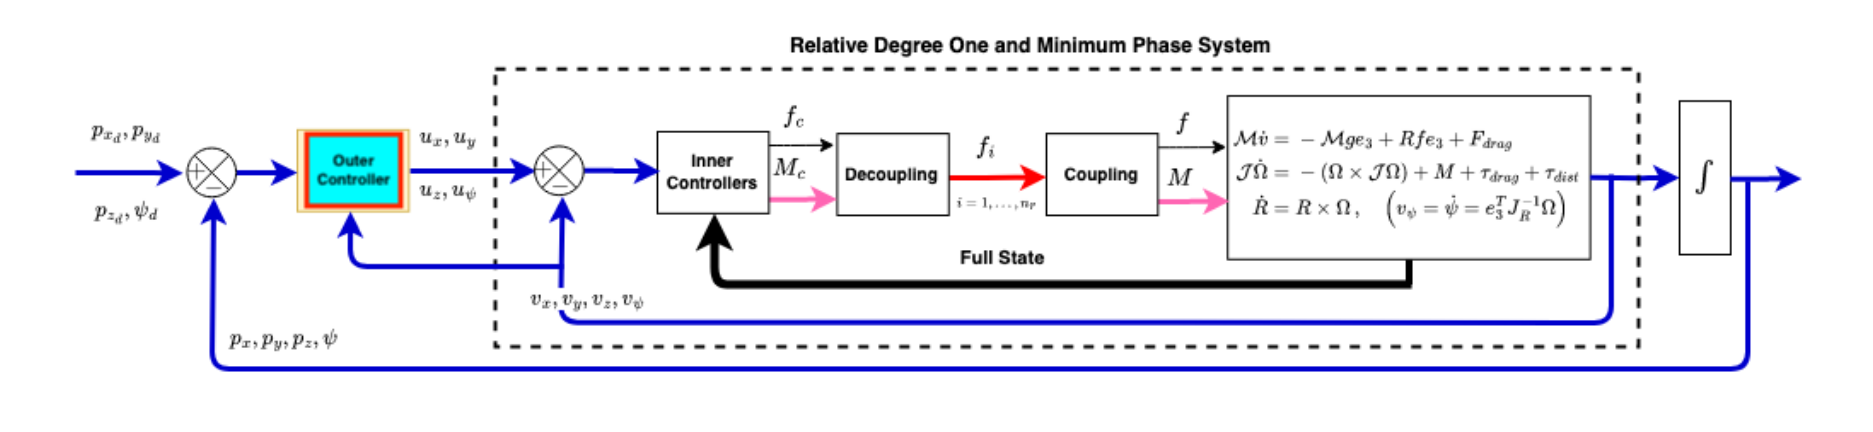
\includegraphics[width=\textwidth]{figs/full_controller.png}
    \caption{Diagrama de Controle}
  \end{figure}
\end{frame}
\begin{frame}{Arquitetura de Controle}
  \begin{columns}[t]
    \column{0.5\textwidth}
      \textbf{Malha externa (posição)}
      \begin{itemize}
        \item Erro de posição + \textit{feedforward} da trajetória.
        \item Gera velocidades desejadas $v_{xd}, v_{yd}, v_{zd}$.
      \end{itemize}
    \column{0.5\textwidth}
      \textbf{Malha interna (atitude/velocidade)}
      \begin{itemize}
        \item Controle de altitude (empuxo $f$).
        \item Controle XY acoplado ao de atitude ($\phi_d, \theta_d$).
        \item Controle de guinada ($\psi$).
      \end{itemize}
  \end{columns}
  \vspace{0.5cm}
  % TODO: diagrama de blocos da arquitetura (malha externa -> interna -> planta)
\end{frame}

\begin{frame}[fragile]{Malha Externa — Lei de Controle}
  Velocidade desejada = ganho proporcional $\times$ erro + termo feedforward:
\begin{lstlisting}
vx_d = KPO * (x_d - state[0]) + self.dot_x_d
vy_d = KPO * (y_d - state[1]) + self.dot_y_d
vz_d = 2*KPO * (z_d - state[2]) + self.dot_z_d
\end{lstlisting}

  % TODO: comentar a escolha do ganho 2x no eixo z
\end{frame}

\begin{frame}{Sintonia Hierárquica dos Ganhos}
  \begin{enumerate}
    \item Ajusta-se primeiro a malha \textbf{interna}.
    \item Somente após estabilizada, afina-se a malha \textbf{externa}.
  \end{enumerate}
  Polinômio característico de 2ª ordem:
  \begin{equation}
    s^2 + K_d s + K_p = 0
    \quad\Longleftrightarrow\quad
    s^2 + 2\zeta\omega_n s + \omega_n^2 = 0
  \end{equation}
  \begin{equation}
    K_p = \omega_n^2, \qquad K_d = 2\zeta\omega_n
  \end{equation}
  Com amortecimento crítico ($\zeta = 1$) e critério de 2\%:
  \begin{equation}
    t_{\text{sub}} \approx \frac{4}{\zeta\omega_n}
    \;\Longrightarrow\; K_d = \frac{8}{t_{\text{sub}}}
  \end{equation}
\end{frame}

\begin{frame}{Linearização por Realimentação — Altitude}
  Cancela as não linearidades da dinâmica vertical
  $\dot{p}_z = -g + (\cos\phi\cos\theta)\mathcal{M}^{-1}f + \mathcal{D}_z$:
  \begin{equation}
    f = \frac{\mathcal{M}\,(\mathcal{U}_z + g)}{\cos\phi\,\cos\theta}
  \end{equation}
  Resultado: dinâmica de malha fechada linear e desacoplada,
  $\dot{p}_z = \mathcal{U}_z + \mathcal{D}_z$.
\end{frame}

\begin{frame}{Linearização por Realimentação — Atitude}
  Anulação dos torques de Coriolis/giroscópicos:
  \begin{align}
    J_{bx}^{-1}M_x &= \dot{\theta}\dot{\psi}(J_{az}-J_{ay}) + \mathcal{U}_\phi \\
    J_{by}^{-1}M_y &= \dot{\phi}\dot{\psi}(J_{ax}-J_{az}) + \mathcal{U}_\theta \\
    J_{bz}^{-1}M_z &= \dot{\theta}\dot{\phi}(J_{ay}-J_{ax}) + \mathcal{U}_\psi
  \end{align}
  $\mathcal{U}_\phi, \mathcal{U}_\theta, \mathcal{U}_\psi$: esforços virtuais (leis PD/PI).
\end{frame}


\begin{frame}{Linearização Direta nos Ângulos}
  Leis de linearização por realimentação (dependentes dos parâmetros):
  \begin{equation}
    J_{bx}^{-1}M_x = \dot{\theta}\dot{\psi}\,(J_{az}-J_{ay}) + \mathcal{U}_\phi,
    \qquad
    J_{by}^{-1}M_y = \dot{\phi}\dot{\psi}\,(J_{ax}-J_{az}) + \mathcal{U}_\theta
  \end{equation}
  resultando na malha fechada linear e desacoplada:
  \begin{equation}
    \ddot{\phi} = \mathcal{U}_\phi + \mathcal{D}_{\Omega_x},
    \qquad
    \ddot{\theta} = \mathcal{U}_\theta + \mathcal{D}_{\Omega_y}
  \end{equation}
  Esforços PD (sem \textit{feedforward} nem ação integral):
  \begin{equation}
    \mathcal{U}_\phi = -k_p^\phi(\phi-\phi_d) - k_d^\phi\,\dot{\phi},
    \qquad
    \mathcal{U}_\theta = -k_p^\theta(\theta-\theta_d) - k_d^\theta\,\dot{\theta}
  \end{equation}
  \begin{equation}
    \ddot{\phi} + k_d^\phi\,\dot{\phi} + k_p^\phi\,\phi
      = k_p^\phi\,\phi_d + \mathcal{D}_{\Omega_x}
    \;\;\Rightarrow\;\;
    \text{erro de rastreamento de ordem } \mathcal{O}(1/k_p^\phi)
  \end{equation}
  (análogo para $\theta$).
\end{frame}

\begin{frame}{Cap.\ 6.3 — Malha Interna de Atitude e Sintonia}
  \begin{figure}
    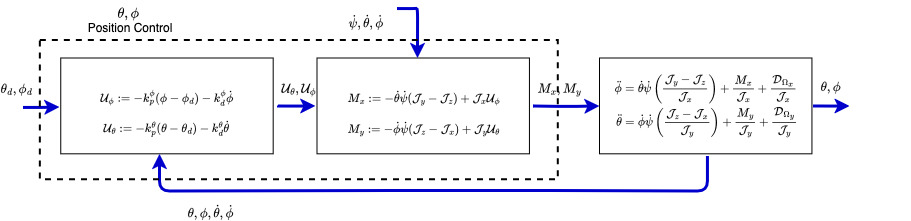
\includegraphics[width=\textwidth]{figs/fig9_roll_pitch_loops.png}
    \caption{Malhas internas de posição de roll e pitch (Fig.\ 9 do documento).}
  \end{figure}
  Sintonia (Remarks 8 e 9): alocação de polos com dinâmica dominante $s + a_p = 0$,
  \begin{equation}
    s^2 + k_d\,s + k_p = (s + a_p)(s + N a_p)
    \;\Longrightarrow\;
    k_d = (N+1)\,a_p, \quad k_p = N a_p^{2}, \quad N > 1
  \end{equation}
\end{frame}

\begin{frame}[fragile]{Cap.\ 6.3 — Implementação (\texttt{control.py})}
\begin{lstlisting}
U_phi   = KP_PHI   * (phi_d - phi)     - KD_PHI   * p
U_theta = KP_THETA * (theta_d - theta) - KD_THETA * q

tau_phi   = q*r*(Jja[2,2]-Jja[1,1]) + U_phi  *Jjb[0,0]
tau_theta = p*r*(Jja[0,0]-Jja[2,2]) + U_theta*Jjb[1,1]
\end{lstlisting}
  \begin{itemize}
    \item $p, q \approx \dot\phi, \dot\theta$ sob ângulos pequenos (filtro
          passa-baixas de 30 Hz disponível para $p$ e $q$).
    \item Termos $qr\,(J_{az}-J_{ay})$ e $pr\,(J_{ax}-J_{az})$: compensação dos
          torques giroscópicos da linearização por realimentação.
    \item Ganhos: $k_p^\phi = k_p^\theta = 100$, $k_d^\phi = k_d^\theta = 20$
          $\Rightarrow$ $\omega_n = 10$ rad/s e $\zeta = 1$
          (amortecimento crítico) na malha de atitude.
  \end{itemize}
\end{frame}

\begin{frame}{Controle de Velocidade $(x,y)$ (Cap.\ 6.4) — Formulação}
  Dinâmica horizontal reescrita evidenciando a direção do empuxo:
  \begin{equation}
    \begin{bmatrix} \ddot{p}_x \\ \ddot{p}_y \end{bmatrix}
    = R_\psi
    \begin{bmatrix} \sin\theta\cos\phi \\ -\sin\phi \end{bmatrix}
    \mathcal{M}^{-1} f
    + \begin{bmatrix} \mathcal{D}_x \\ \mathcal{D}_y \end{bmatrix},
    \qquad
    R_\psi =
    \begin{bmatrix} \cos\psi & -\sin\psi \\ \sin\psi & \cos\psi \end{bmatrix}
  \end{equation}
  Ideia: escolher os ângulos desejados de modo que a projeção do empuxo
  realize o esforço virtual $\mathcal{U} = [\mathcal{U}_x, \mathcal{U}_y]^T$:
  \begin{equation}
    \begin{bmatrix} \sin\theta_d\cos\phi_d \\ -\sin\phi_d \end{bmatrix}
    = R_\psi^{-1}\,\mathcal{U}\,\mathcal{M} f^{-1}
  \end{equation}
  Se as malhas de atitude garantem $\theta \approx \theta_d$ e $\phi \approx \phi_d$:
  \begin{equation}
    \begin{bmatrix} \ddot{p}_x \\ \ddot{p}_y \end{bmatrix}
    \;\approx\; \mathcal{U} + \begin{bmatrix} \mathcal{D}_x \\ \mathcal{D}_y \end{bmatrix}
  \end{equation}
  Ou seja: \textbf{o controle de posição horizontal é feito inclinando o veículo}
  — a malha $(x,y)$ gera referências para a malha de atitude.
\end{frame}

\begin{frame}{Cap.\ 6.4 — Esforços PI com Feedforward}
  $\mathcal{U}_x$ e $\mathcal{U}_y$ são esforços PI que rastreiam as
  velocidades de referência $u_x = \dot{p}_{xd}$ e $u_y = \dot{p}_{yd}$
  (vindas da malha externa):
  \begin{align}
    \mathcal{U}_x &= -k_d^x\,(\dot{p}_x - u_x) + k_{ff}^x\,\dot{u}_x
                     - k_i^x\!\int_0^t (\dot{p}_x - u_x)\,d\tau \\
    \mathcal{U}_y &= -k_d^y\,(\dot{p}_y - u_y) + k_{ff}^y\,\dot{u}_y
                     - k_i^y\!\int_0^t (\dot{p}_y - u_y)\,d\tau
  \end{align}
  \begin{itemize}
    \item $k_{ff} = 1$ quando $\dot{u}$ está disponível; $k_{ff} = 0$ caso contrário.
    \item A ação integral rejeita perturbações constantes (vento) —
          mas, combinada com a saturação dos atuadores, exige \textbf{anti-windup}.
  \end{itemize}
\end{frame}

\begin{frame}[fragile]{Cap.\ 6.4 — Implementação (\texttt{control.py})}
\begin{lstlisting}
U_x = KP_X*self.intgr_e_vx - KD_X*evx + ax_d
U_y = KP_Y*self.intgr_e_vy - KD_Y*evy + ay_d
arr = inv(R_psi) @ [U_x, U_y] * m/f # [sin(th_d)cos(phi_d), -sin(phi_d)]
phi_d   = -arcsin(clip(arr[1], -1, 1))
theta_d =  arcsin(clip(arr[0]/cos(phi_d), -1, 1))
theta_d = clip(theta_d, -MAX_ANGLE, MAX_ANGLE)  # +/- 15 deg
phi_d   = clip(phi_d,   -MAX_ANGLE, MAX_ANGLE)
\end{lstlisting}
  \begin{itemize}
    \item Convenção do código: \texttt{KP\_X} multiplica a \textbf{integral}
          (equivale a $k_i^x$) e \texttt{KD\_X} o erro de velocidade ($k_d^x$);
          $k_{ff} = 1$ realizado por \texttt{ax\_d}, \texttt{ay\_d}.
    \item Saturação de $\pm 15^\circ$: preserva a hipótese de ângulos pequenos e
          limita a aceleração horizontal $\Rightarrow$ motiva o anti-windup.
  \end{itemize}
\end{frame}

\begin{frame}{Cap.\ 6.4 — Malha Fechada e Sintonia}
  \footnotesize
  Substituindo os esforços PI na dinâmica (com $\bar{\mathcal{D}}$: termos
  residuais das malhas de atitude), obtém-se a dinâmica de erro de 3ª ordem:
  \begin{align}
    (\dddot{p}_x - \ddot{u}_x) + k_d^x(\ddot{p}_x - \dot{u}_x) + k_i^x(\dot{p}_x - u_x)
      &= \dot{\mathcal{D}}_x + \dot{\bar{\mathcal{D}}}_x + (k_{ff}^x-1)\,\ddot{u}_x \\
    (\dddot{p}_y - \ddot{u}_y) + k_d^y(\ddot{p}_y - \dot{u}_y) + k_i^y(\dot{p}_y - u_y)
      &= \dot{\mathcal{D}}_y + \dot{\bar{\mathcal{D}}}_y + (k_{ff}^y-1)\,\ddot{u}_y
  \end{align}
  Sintonia (Remark 10), para $j = x, y$: polo dominante em $-a_p^j$,
  \begin{equation*}
    s^2 + k_d^j s + k_i^j = (s + a_p^j)(s + N_j a_p^j)
    \;\Longrightarrow\;
    k_d^j = (N_j+1)\,a_p^j, \quad k_i^j = N_j\,(a_p^j)^{2}
  \end{equation*}
  \begin{figure}
    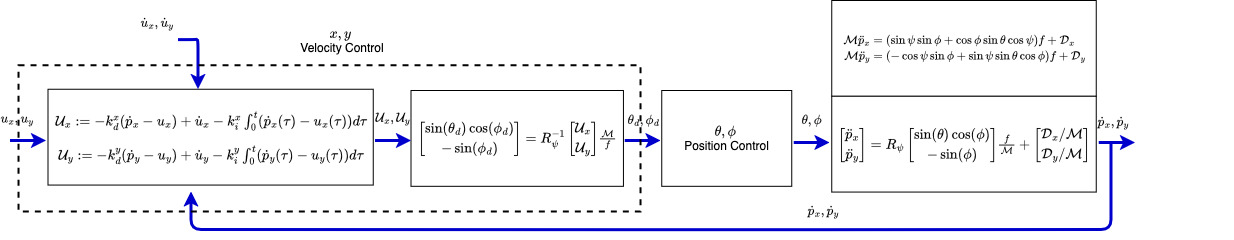
\includegraphics[width=0.92\textwidth]{figs/fig10_xy_velocity_loop.png}
    \caption{Malha interna de velocidade $(x,y)$ (Fig.\ 10 do documento).}
  \end{figure}
\end{frame}

\begin{frame}{Anti-Windup — Formulação Teórica}
  \footnotesize
  Integrador puro: $\dot{x}_i = y$, \; $y_i = x_i$. Com saturação da saída:
  \begin{equation}
    \operatorname{SAT}(x_i) =
    \begin{cases}
      \mathrm{SAT}_{\min}, & x_i \le \mathrm{SAT}_{\min} \\
      x_i,                 & \text{caso contrário} \\
      \mathrm{SAT}_{\max}, & x_i \ge \mathrm{SAT}_{\max}
    \end{cases}
  \end{equation}
  \begin{block}{Integrador com anti-windup por retro-cálculo (\emph{back-calculation})}
    \vspace{-0.4em}
    \begin{equation}
      \dot{x}_i = y + k_{aw}\,[x_i - \operatorname{SAT}(x_i)],
      \qquad
      y_i = \operatorname{SAT}(x_i)
    \end{equation}
    \vspace{-0.6em}
    \begin{itemize}
      \item Dentro dos limites: $x_i - \operatorname{SAT}(x_i) = 0$
            $\Rightarrow$ integrador nominal, sem alteração.
      \item Saturado: o termo de retro-cálculo ($k_{aw} < 0$) \textbf{puxa $x_i$
            de volta} à faixa linear, impedindo o acúmulo (\emph{windup}).
    \end{itemize}
  \end{block}
  Versão discreta (Euler, período de amostragem $h$) — eqs.\ (145)--(146) do documento:
  \begin{equation}
    y_i[k] = \operatorname{SAT}(x_i[k]),
    \qquad
    x_i[k+1] = x_i[k] + h\,\big(y[k] + k_{aw}\,[x_i[k] - \operatorname{SAT}(x_i[k])]\big)
  \end{equation}
\end{frame}

\begin{frame}[fragile]{Anti-Windup — Implementação (\texttt{control.py})}
\begin{lstlisting}
L = self.intgr_limit   # 0.5
self.mem_intgr_e_vx += dt*( e_vx - k_aw*( intgr_e_vx
                            - clip(mem_intgr_e_vx, -L, L) ) )
self.intgr_e_vx = clip(self.mem_intgr_e_vx, -L, L)  # y_i = SAT(x_i)
\end{lstlisting}
  \begin{itemize}
    \item Correspondência com a teoria: estado do integrador
          $x_i \leftrightarrow$ \texttt{mem\_intgr\_e\_v*}; saída saturada
          $y_i = \operatorname{SAT}(x_i) \leftrightarrow$ \texttt{intgr\_e\_v*}
          (via \texttt{clip}); discretização de Euler com $h = \Delta t_{\text{sim}}$.
    \item $k_{aw} = 2{,}0$ (o sinal negativo na atualização equivale ao
          $k_{aw} < 0$ da formulação contínua); limites $\pm 0{,}5$.
    \item \textbf{Por que é necessário:} o empuxo satura em
          $[0{,}25\,\mathcal{M}g,\; 2\,\mathcal{M}g]$ e os ângulos em $\pm 15^\circ$.
          Sob o vento de 3 N em $x$, o canal $\theta$ satura (conforme nota no
          código); sem anti-windup, a integral seguiria crescendo durante a
          saturação, causando \emph{overshoot} e recuperação lenta.
  \end{itemize}
\end{frame}


% ============================================================
% 4. SIMULAÇÃO
% ============================================================
\section{Arquitetura de Simulação}
\begin{frame}[fragile]{Ambiente de Simulação}
  \begin{itemize}
    \item Python + \texttt{scipy.integrate.solve\_ivp} (RK45).
    \item Vetor de estados: 12 estados (posição, velocidade, ângulos de Euler,
          velocidades angulares)
    \item Núcleo: função \texttt{closed\_loop\_dynamics}.
  \end{itemize}
 \vspace{0.3cm} 
  \textbf{Configurações do Drone}
\begin{minted}{python}
g = 9.81
m = 1.5  # drone mass [kg]
d_uav = 0.2 # drone radius [m]
h_uav = 0 # drone height [m]
J = np.diag([
    0.025,  # Jx
    0.025,  # Jy
    0.045   # Jz
])

\end{minted}
% TODO: tabela de parâmetros do VANT simulado (massa, inércias, etc.)
\end{frame}

\begin{frame}{Fluxo de Execução (Closed-Loop)}
  \begin{enumerate}
    \item \textbf{Geração de trajetória:} interpola $(x_d, y_d, z_d)$.
    \item \textbf{Malha externa:} erro de posição $\to$ velocidades desejadas.
    \item \textbf{Controle de altitude:} $f = \dfrac{\mathcal{M}(g+\mathcal{U}_z)}{\cos\phi\cos\theta}$.
    \item \textbf{Controle XY:} extrai $\phi_d, \theta_d$ via $R_\psi^{-1}$.
    \item \textbf{Controle de atitude:} torques $(\tau_\phi, \tau_\theta, \tau_\psi)$.
    \item \textbf{Planta:} Newton--Euler 6-DOF $\to$ $\dot{x}$ para o integrador.
  \end{enumerate}
  
  % TODO: fluxograma do loop de simulação
\end{frame}

\begin{frame}{Robustez na Simulação}
  \begin{itemize}
    \item \textbf{Anti-windup} por retro-cálculo na lei de controle
    \item \textbf{Injeção de distúrbios:} força externa estática (vento) em
          janela de tempo, atuando como aceleração parasita nas velocidades.
    \item \textbf{Zero Order Hold:} física e controle alternados em loop,
          emulando um microcontrolador real. Ambos a 200Hz
  \end{itemize}
  % TODO: detalhar taxa de amostragem do ZOH e janela do distúrbio
\end{frame}



\begin{frame}{Simulações realizadas e Métricas}
  \begin{columns}[t]
    \column{0.55\textwidth}
      \textbf{Trajetórias}
      \begin{itemize}
        \item  Degrau em $y$ + Rampa em $z$
        \begin{itemize}
            \item X: 0
            \item Y: 1m
            \item Z: 1m/s
        \end{itemize}
        \item Circular livre
            \begin{itemize}
            \item Raio = 2m
            \item $\omega = \frac{1}{2} rad/s$
            \end{itemize}
        \item Circular com vento (2, 0, 2)N
            \begin{itemize}
            \item Raio = 2m
            \item $\omega = \frac{1}{2} rad/s$
            \end{itemize}
        \item Circular com vento (2, 0, -2)N
            \begin{itemize}
            \item Raio = 2m
            \item $\omega = \frac{1}{2} rad/s$
            \end{itemize}

      \end{itemize}
    \column{0.45\textwidth}
      \textbf{Métricas}
      \begin{itemize}
        \item Ultrapassagem (\textit{overshoot})
        \item Tempo de acomodação
        \item Tempo de resposta a perturbação
      \end{itemize}
  \end{columns}
\end{frame}

% ============================================================
% 5. RESULTADOS
% ============================================================
\section{Resultados}

\begin{frame}{Resultados — Degrau em $y$ + Rampa em $z$}
  Trajetória: Degrau Y, Rampa Z; Perrturbação: (2,0,-2)
    \begin{columns}[c]
      % Coluna da Esquerda: Gráficos
      \column{0.6\textwidth}
        \begin{figure}
          \centering
          % Ajuste o nome da figura gerada pelo seu script
          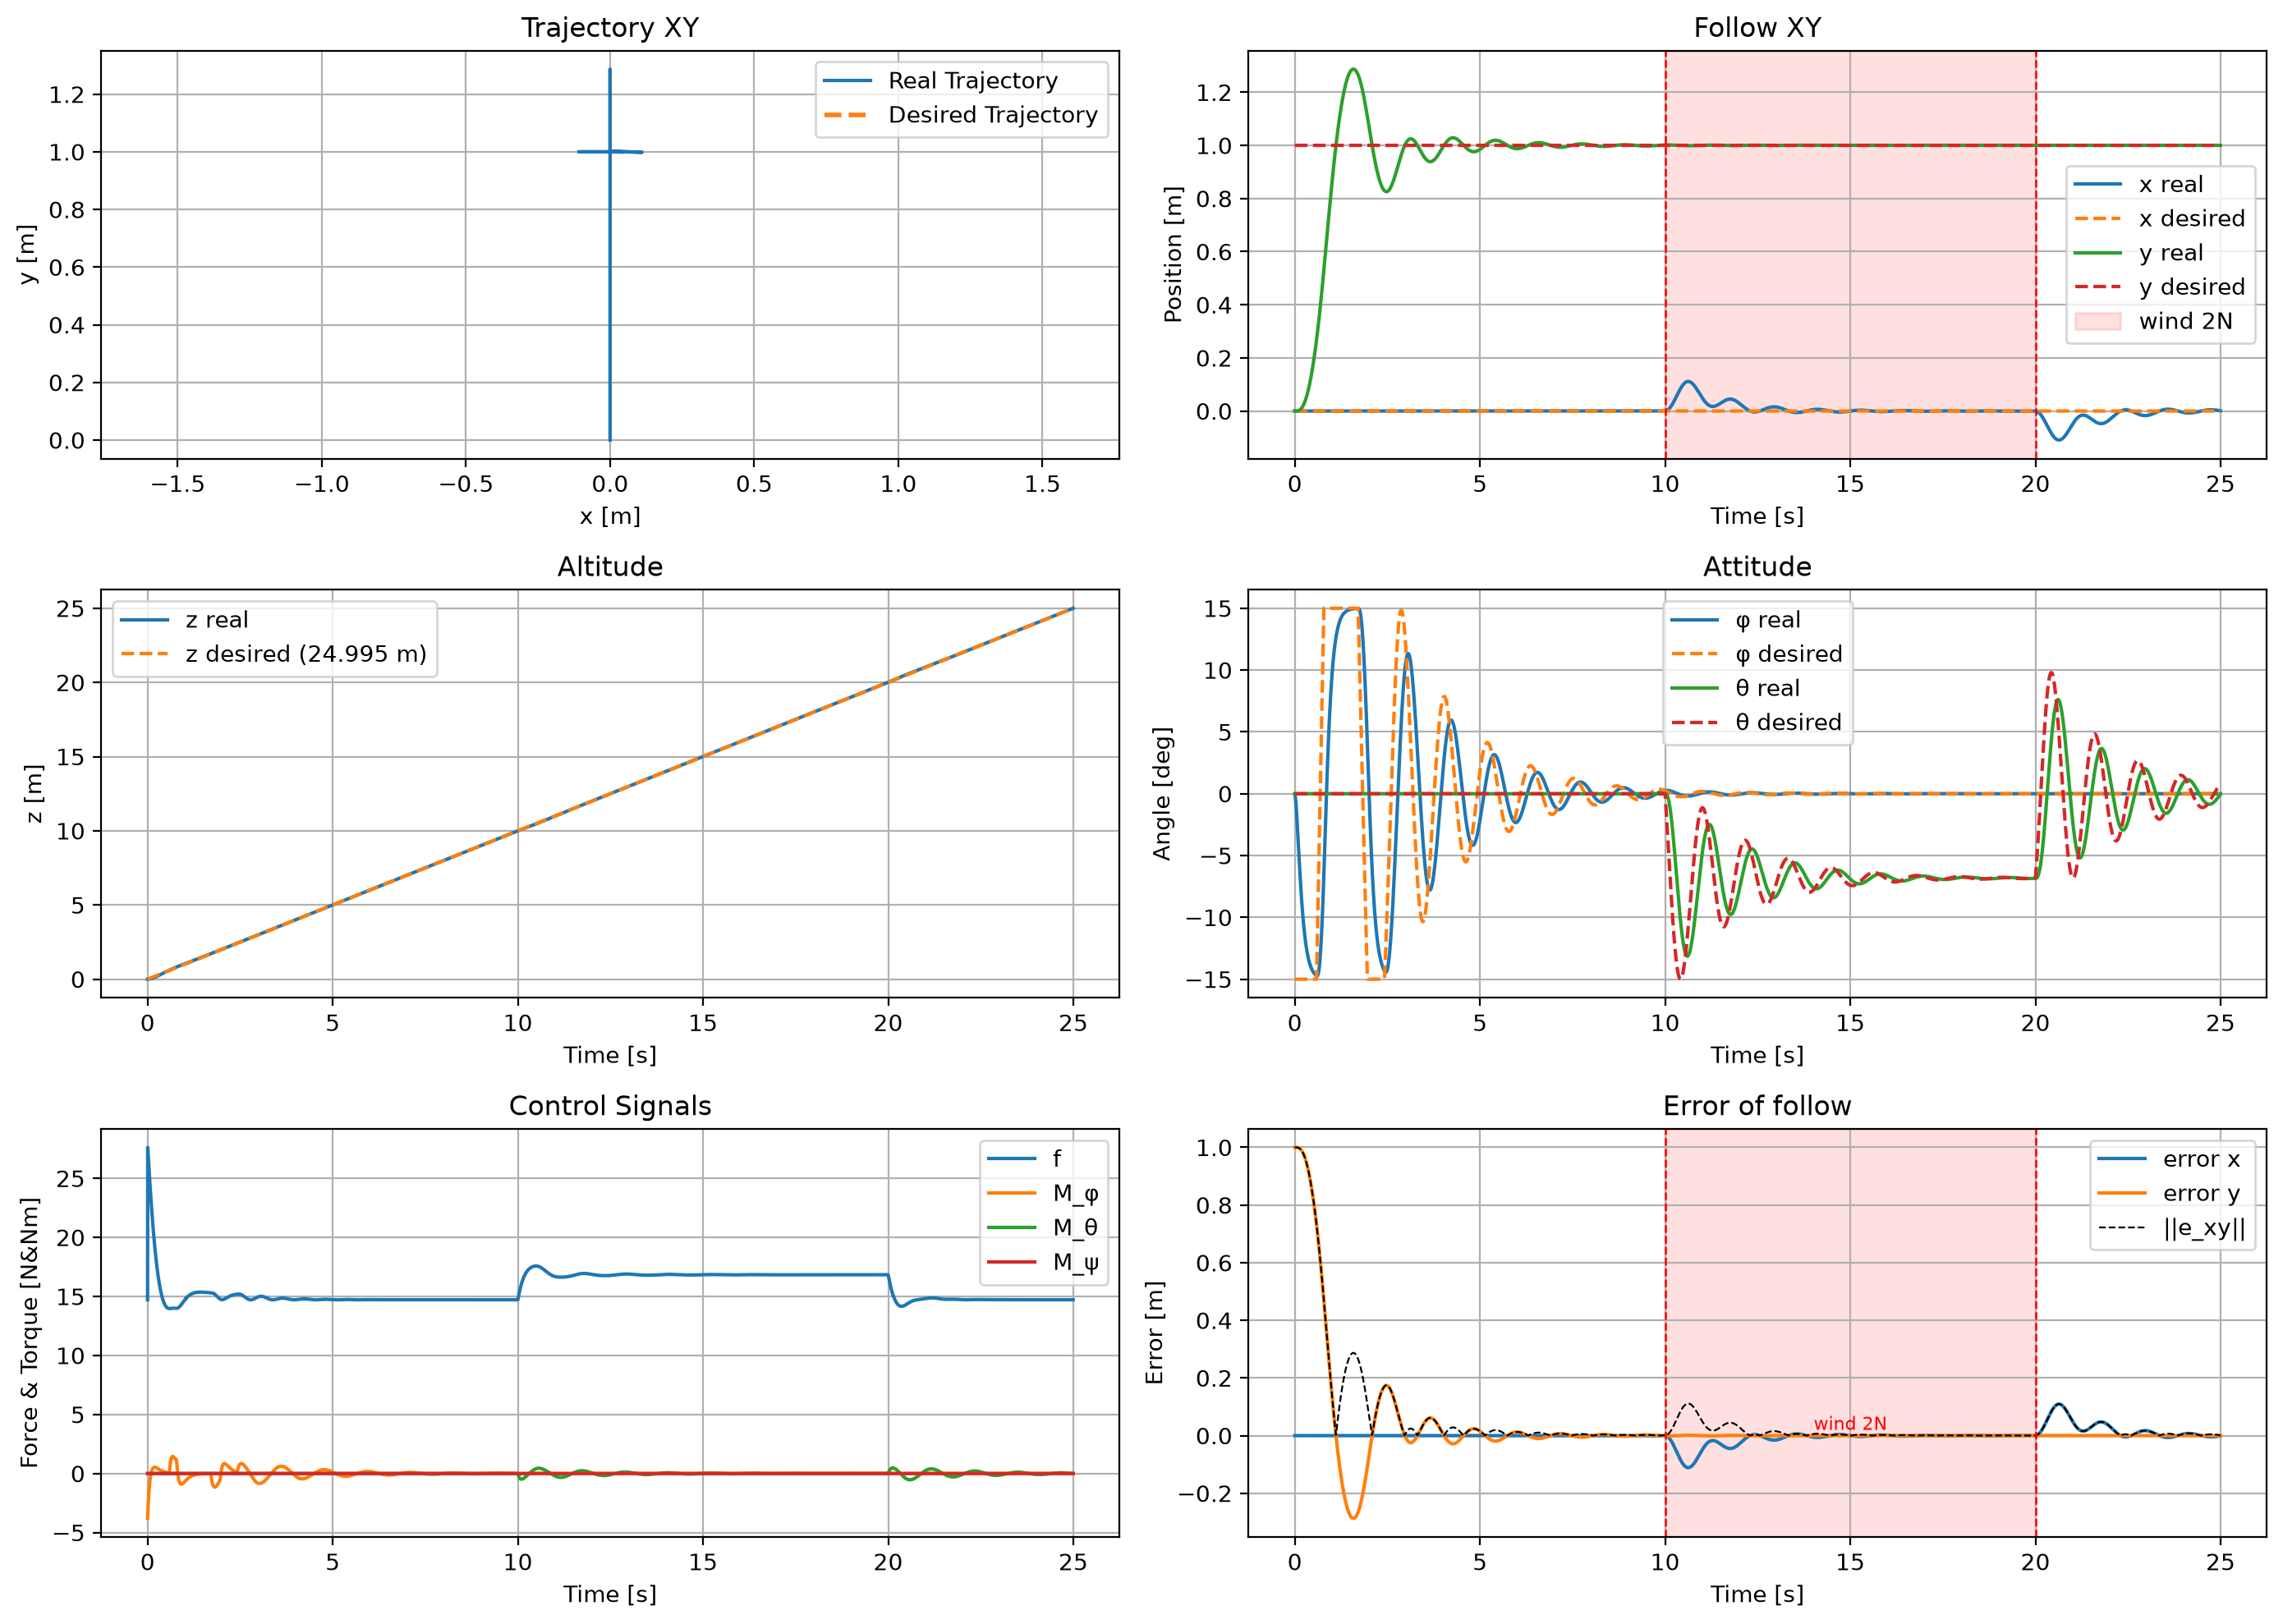
\includegraphics[width=\textwidth]{Figures/line -2z.png} 
        \end{figure}
        
      % Coluna da Direita: Métricas exportadas
      \column{0.4\textwidth}
        \textbf{Desempenho Medido:}\\
        \vspace{0.3cm}
        \footnotesize % Reduz o tamanho da fonte para caber bem
        \begin{itemize}
  \item \textbf{Eixo Z (Altitude):}
  \begin{itemize}
    \item Overshoot: 0.0\%
    \item Tempo de subida: -  
  \end{itemize}
  \item \textbf{Plano XY:}
  \begin{itemize}
    \item Erro xy Overshoot: 0.25 m
    \item Tempo convergência: 2.73s (limiar <= 0.1 m)
    \item Erro em regime X: 2.39 cm
    \item Erro em regime Y: 0.00 cm
  \end{itemize}
\end{itemize}
 % Importa o arquivo gerado pelo Python
    \end{columns}
\end{frame}
\begin{frame}{Resultados — Trajetória Circular Livre}
  \begin{columns}[c]
    % Coluna da Esquerda: Gráficos
    \column{0.6\textwidth}
      \begin{figure}
        \centering
        % Ajuste o nome da figura gerada pelo seu script
        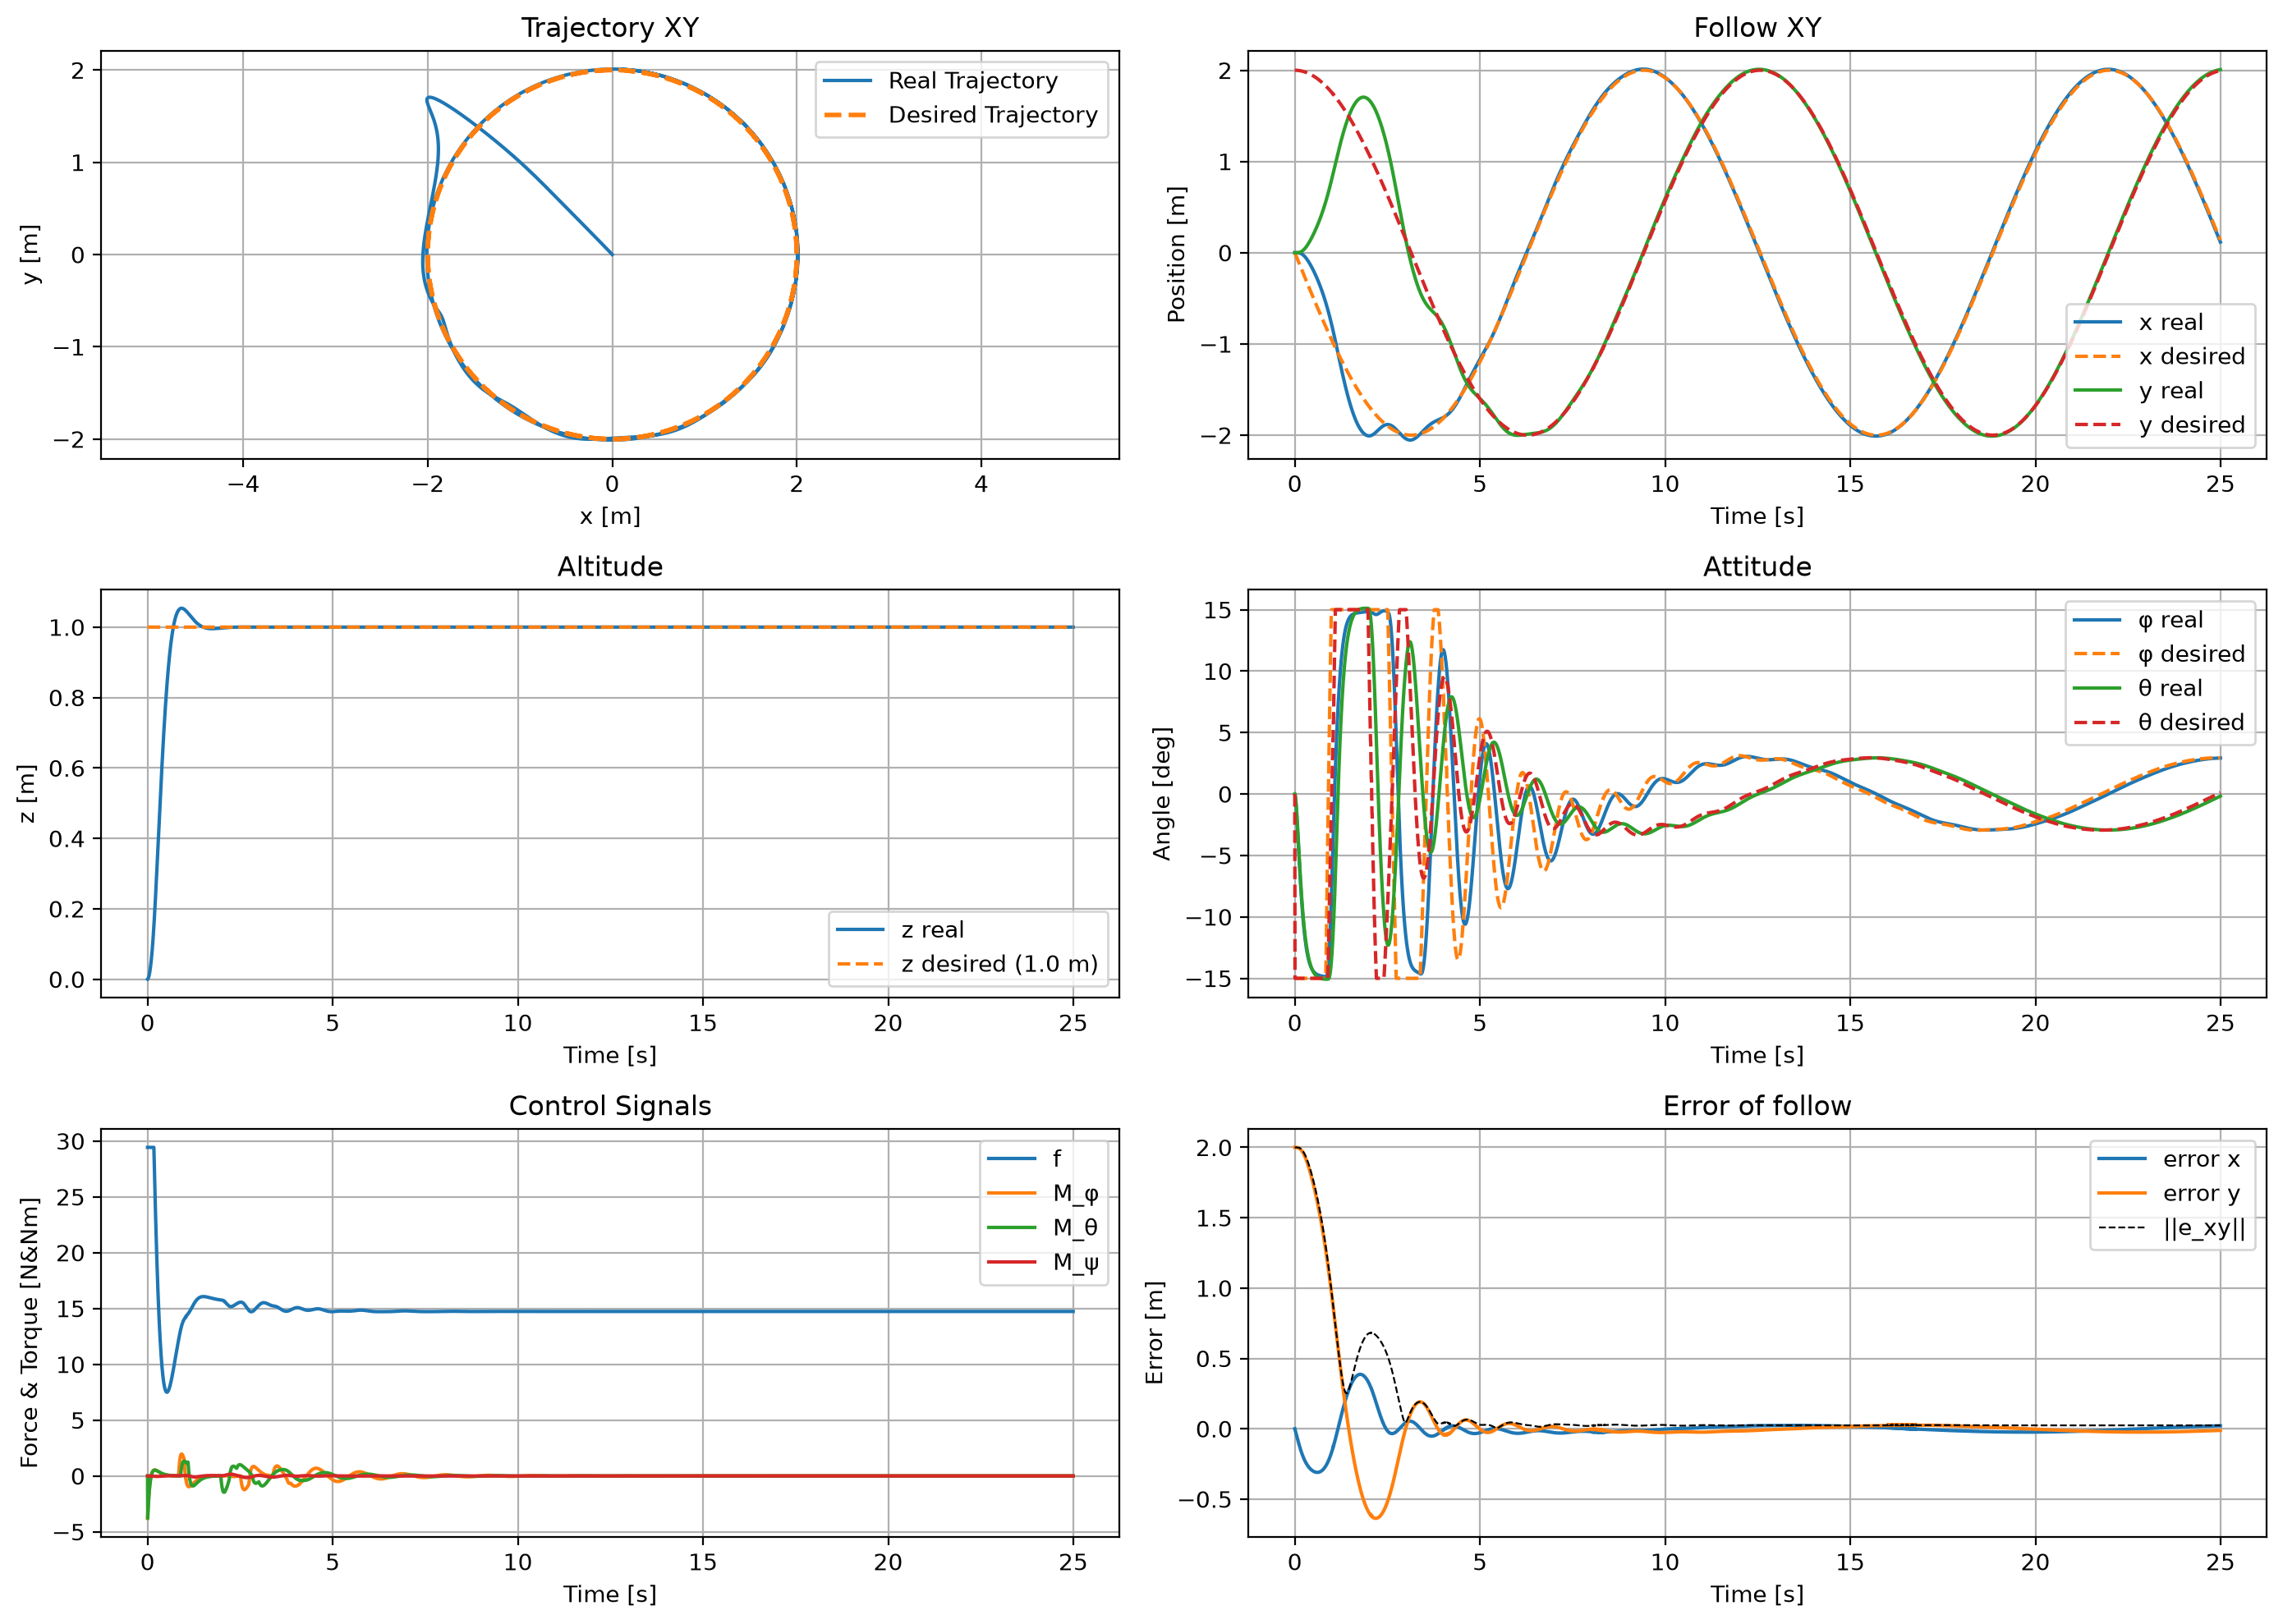
\includegraphics[width=\textwidth]{Figures/circ_livre.png} 
      \end{figure}
      
    % Coluna da Direita: Métricas exportadas
    \column{0.4\textwidth}
      \textbf{Desempenho Medido:}\\
      \vspace{0.3cm}
      \footnotesize % Reduz o tamanho da fonte para caber bem
      \begin{itemize}
  \item \textbf{Eixo Z (Altitude):}
  \begin{itemize}
    \item \textit{Overshoot:} 5.4\%
    \item Tempo de subida: 0.44 s
    \item Erro em regime: 0.00 cm
  \end{itemize}
  \item \textbf{Plano XY:}
  \begin{itemize}
    \item Erro xy Overshoot: 0.682 m
    \item Tempo convergência: 2.81 s
    \item Erro em regime X: 1.32 cm
    \item Erro em regime Y: 1.79 cm
  \end{itemize}
\end{itemize}
 % Importa o arquivo gerado pelo Python
  \end{columns}
\end{frame}
\begin{frame}{Resultados — Trajetória Circular Perturbada (2,0,2)}
  \begin{columns}[c]
    % Coluna da Esquerda: Gráficos
    \column{0.6\textwidth}
      \begin{figure}
        \centering
        % Ajuste o nome da figura gerada pelo seu script
        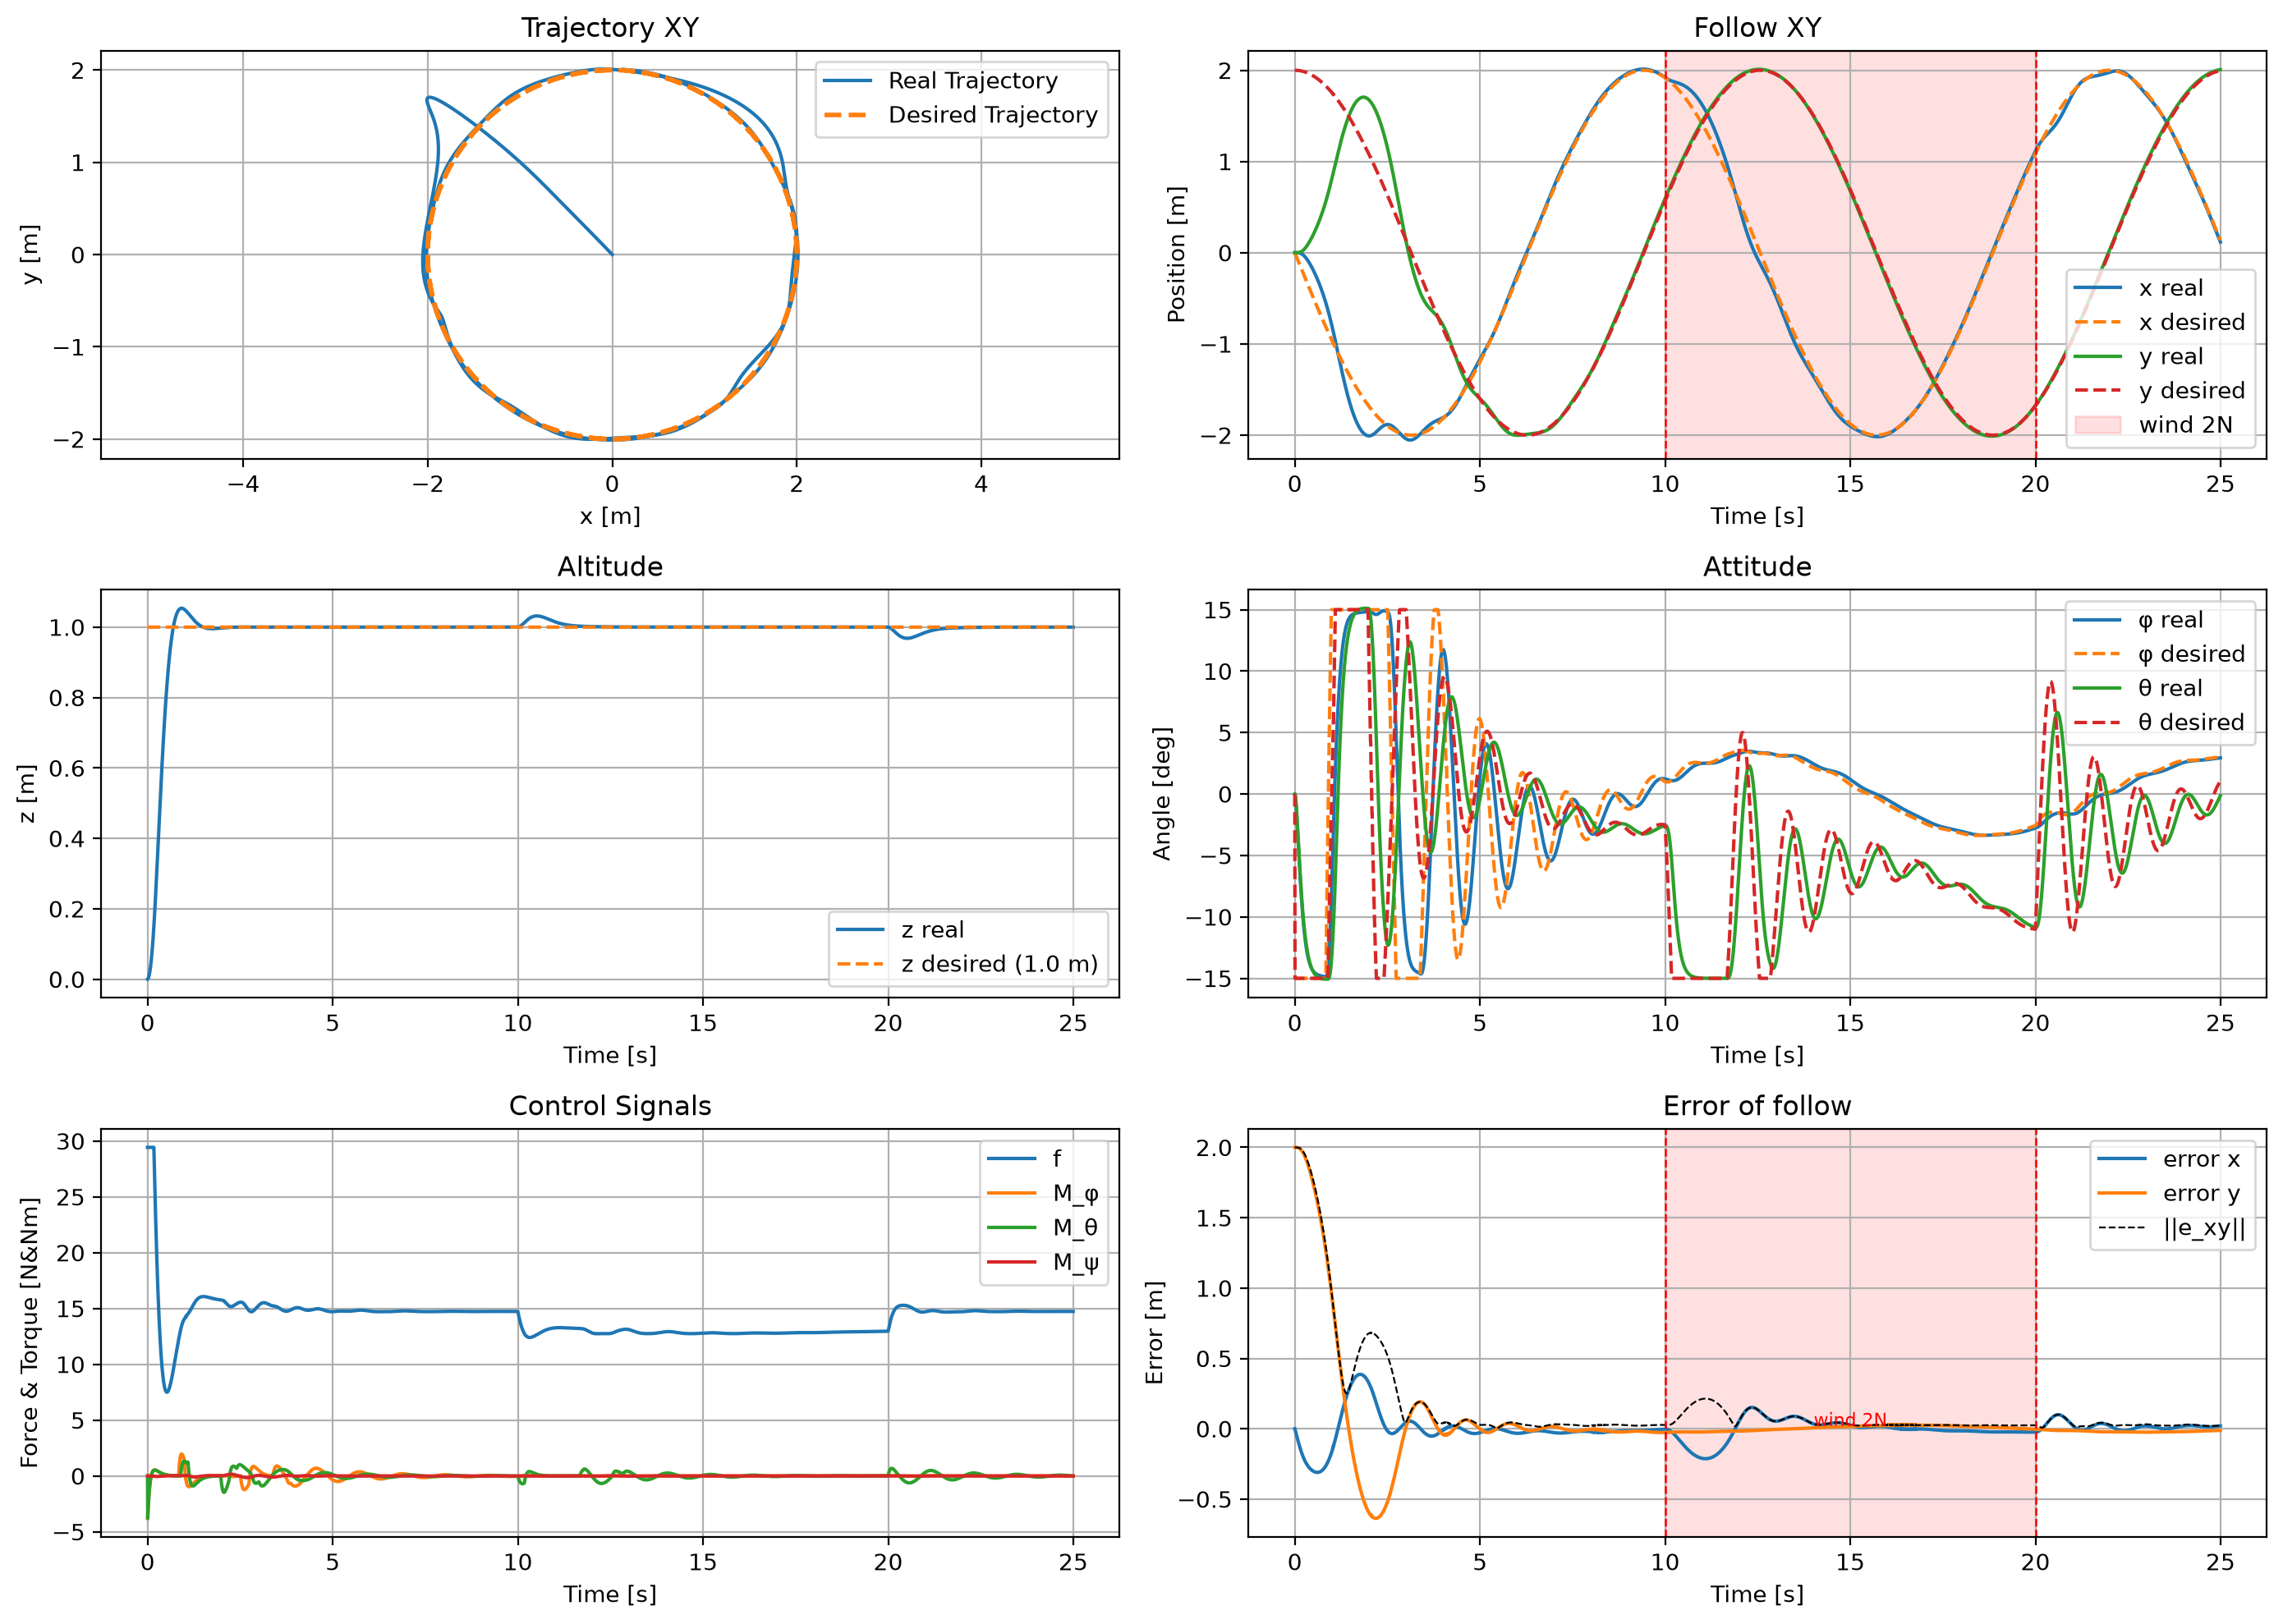
\includegraphics[width=\textwidth]{Figures/circ_vento.png} 
      \end{figure}
      
    % Coluna da Direita: Métricas exportadas
    \column{0.4\textwidth}
      \textbf{Desempenho Medido:}\\
      \vspace{0.3cm}
      \footnotesize % Reduz o tamanho da fonte para caber bem
      \begin{itemize}
  \item \textbf{Eixo Z (Altitude):}
  \begin{itemize}
    \item Overshoot: 5.4\%
    \item Tempo de subida: 0.44 s
  \end{itemize}
  \item \textbf{Plano XY:}
  \begin{itemize}
    \item Erro xy Overshoot: 0.682 m
    \item Tempo convergência: 2.81 s
    \item Erro em regime X: 2.25 cm
    \item Erro em regime Y: 1.79 cm
  \end{itemize}
\end{itemize}
 % Importa o arquivo gerado pelo Python
  \end{columns}
\end{frame}
\begin{frame}{Resultados — Trajetória Circular Perturbada (2,0,-2)}
  \begin{columns}[c]
    % Coluna da Esquerda: Gráficos
    \column{0.6\textwidth}
      \begin{figure}
        \centering
        % Ajuste o nome da figura gerada pelo seu script
        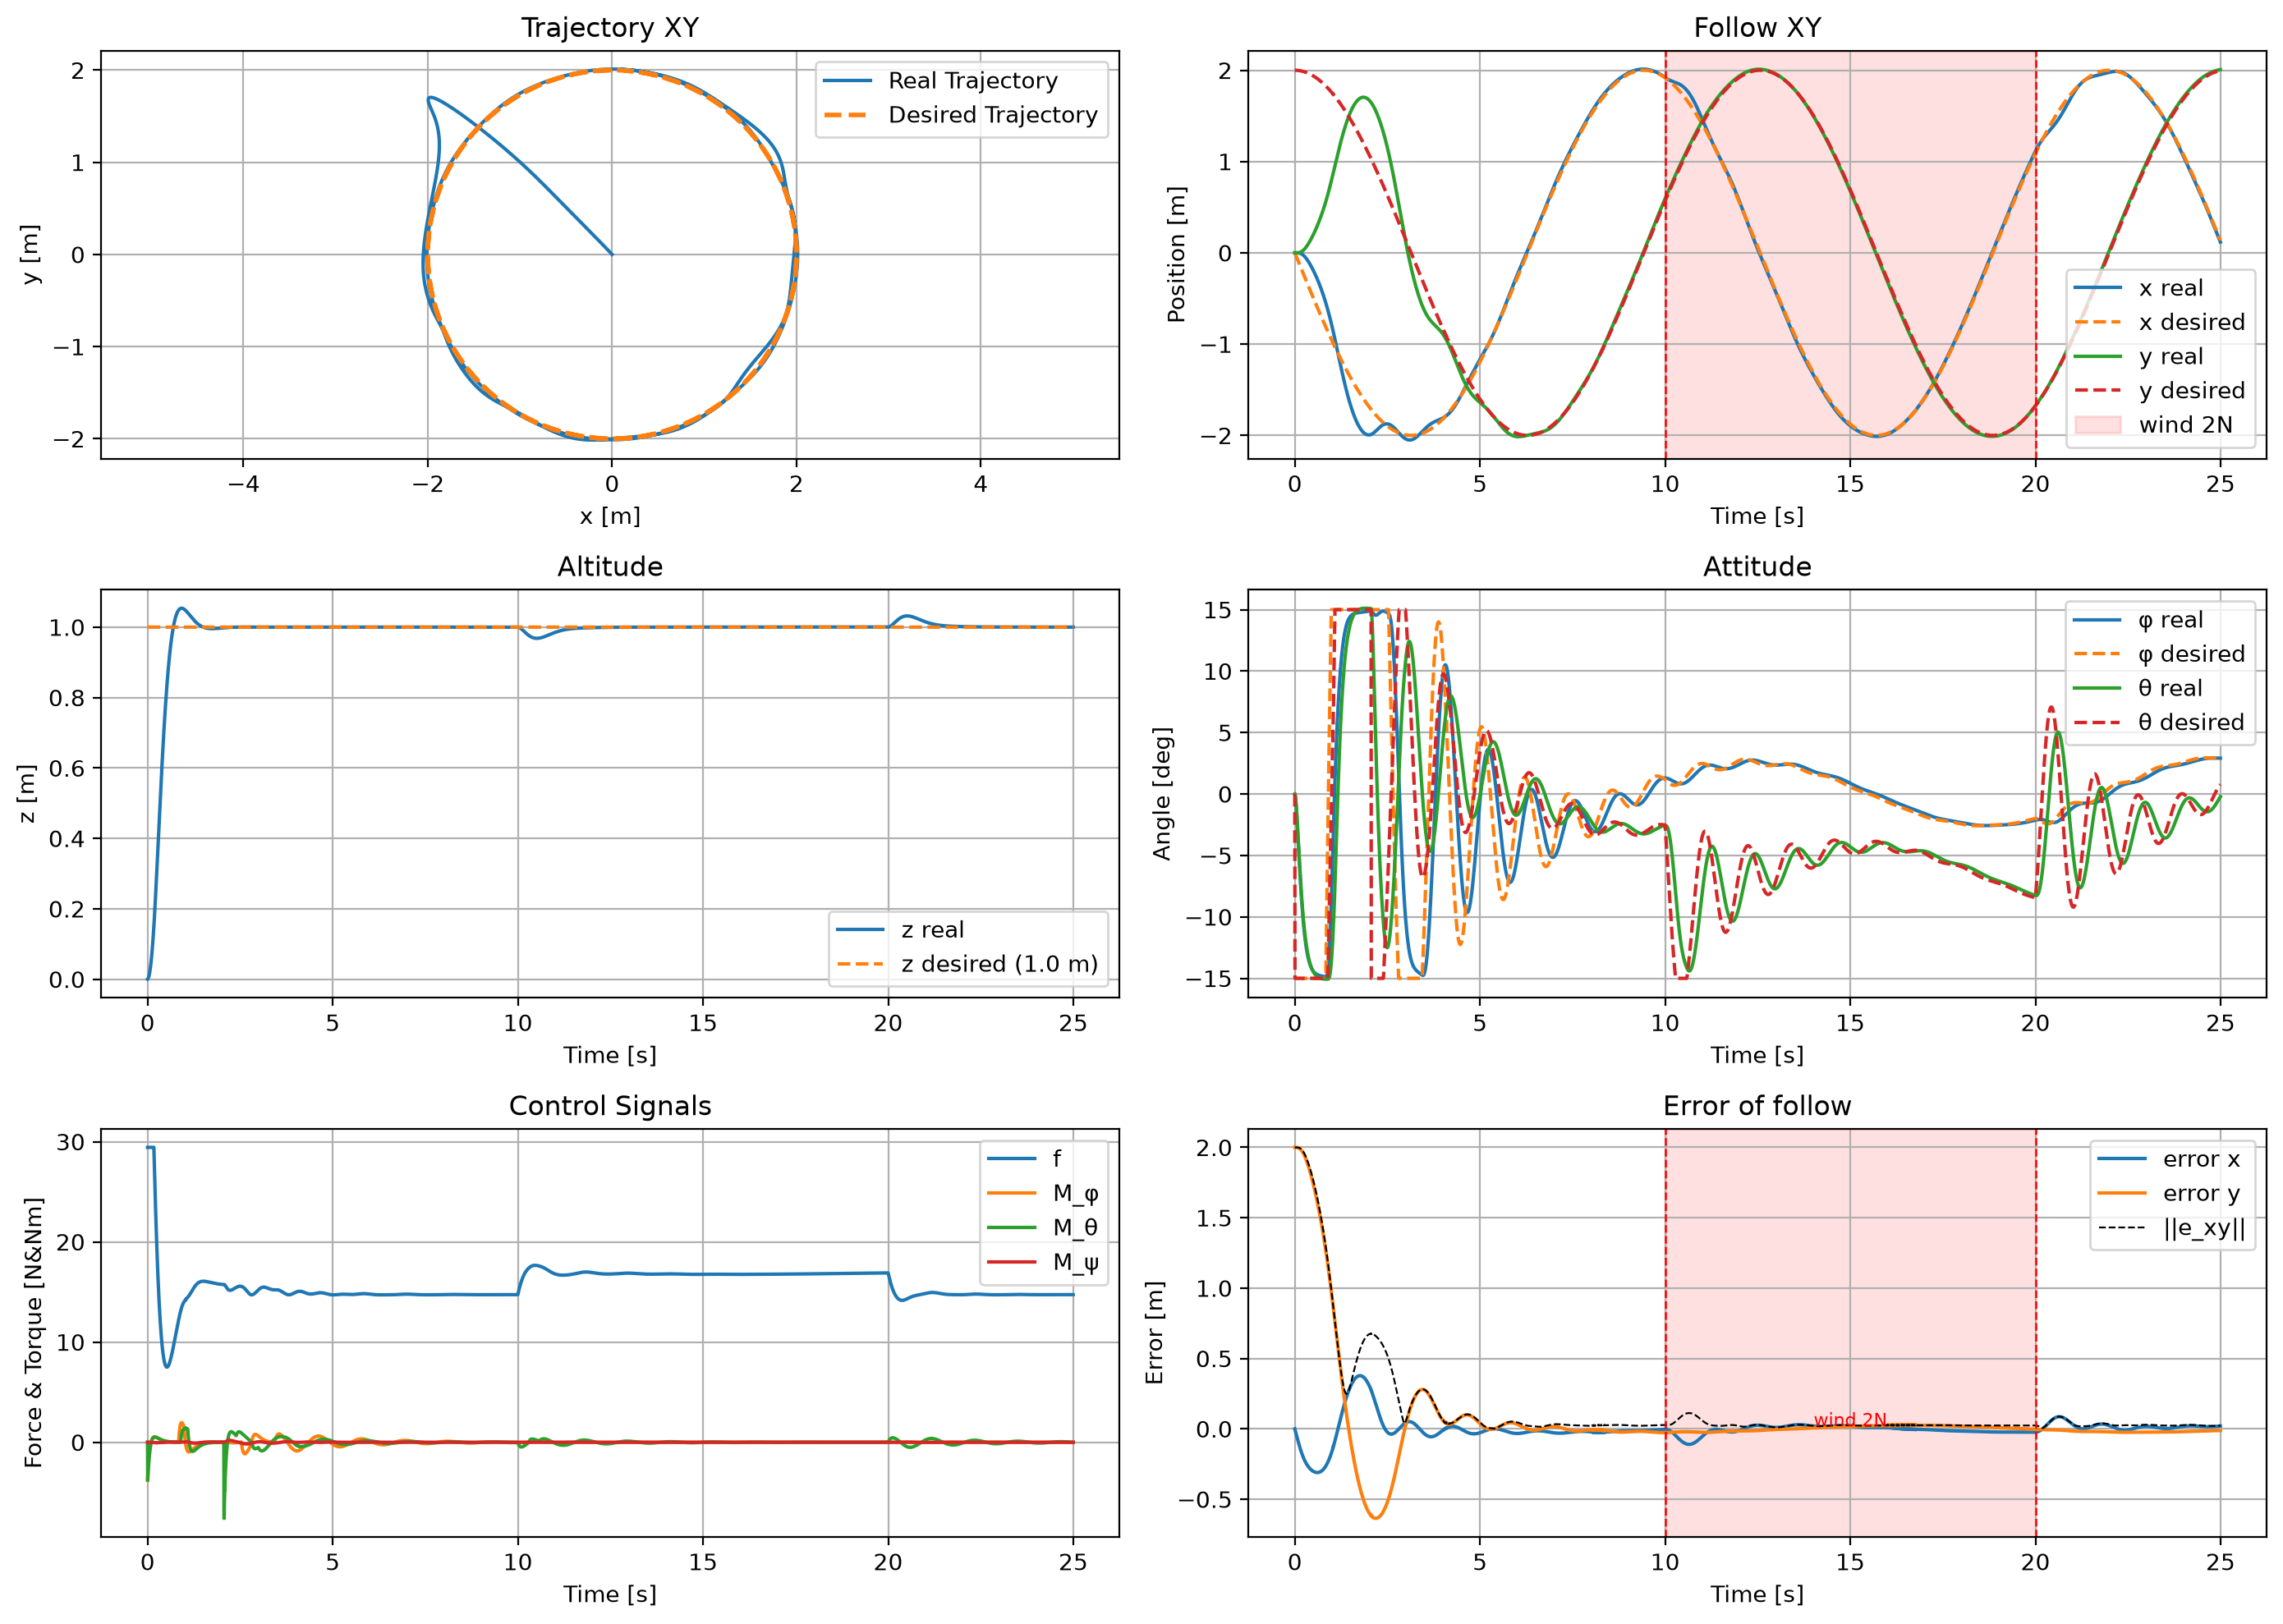
\includegraphics[width=\textwidth]{Figures/cvento -2z.png} 
      \end{figure}
      
    % Coluna da Direita: Métricas exportadas
    \column{0.4\textwidth}
      \textbf{Desempenho Medido:}\\
      \vspace{0.3cm}
      \footnotesize % Reduz o tamanho da fonte para caber bem
      \begin{itemize}
  \item \textbf{Eixo Z (Altitude):}
  \begin{itemize}
    \item Overshoot: 5.4\%
    \item Tempo de subida: 0.44 s
  \end{itemize}
  \item \textbf{Plano XY:}
  \begin{itemize}
    \item Erro xy Overshoot: 0.676 m
    \item Tempo convergência: 3.73 s
    \item Erro em regime X: 2.09 cm
    \item Erro em regime Y: 1.79 cm
  \end{itemize}
\end{itemize}
 % Importa o arquivo gerado pelo Python
  \end{columns}
\end{frame}
  



% ============================================================
% 6. ENCERRAMENTO
% ============================================================
\section{Conclusão}

\begin{frame}{Conclusões e Próximos Passos}
  \textbf{Conclusões}
  \begin{itemize}
    \item Propôs-se uma nova arquitetura de controle com base no modelo dinâmico do drone
    \item Validou-se o controle com a utilização de simulações
    \item Atestou-se a robustez do controle contra forças perturbativas externas
  \end{itemize}
  \textbf{Próximos objetivos}
  \begin{itemize}
    \item Simulação Ros2, Gazebo     
    \item Validação Experimental     
    \item Aplicação de Filtro de Kalman     
    \item Modelagem para velocidades mais altas
  \end{itemize}
\end{frame}

\begin{frame}{Referências}
  \begin{thebibliography}{9}
    \bibitem{peixoto}
      A. J. Peixoto,
      \emph{UAV Modelling and Control}, 2025.
    \bibitem{Erick}
    PFEIFER, Erick. Projeto e controle de um UAV quadrirotor. 2013. Dissertação (Mestrado em Engenharia de Sistemas) - Escola Politécnica, Universidade de São Paulo, São Paulo, 2013. doi:10.11606/D.3.2013.tde-06072014-223705. Acesso em: 2026-10-05.
    % TODO: adicionar demais referências (livros de controle, artigos)
  \end{thebibliography}
\end{frame}

\begin{frame}
  \centering
  \Huge Obrigado!\\[0.5cm]
  \large Perguntas?
\end{frame}

\end{document}